\section{Methodology}\label{sec:method}

\subsection{Evaluation protocol}\label{sec:protocol}
For every corpus and every seed $s\in\{0,\dots,4\}$ we draw a stratified 70/10/20 train/validation/test split. The seed also fixes model initialisation and any subsampling. Training splits are capped at 8{,}000 items, validation at 1{,}500 and test at 3{,}000 (stratified) so that the largest corpora do not dominate run time, and every cap is applied in the same way to every model. Featurisers (vocabularies, IDF weights, SVD bases) are fitted on the source training split only. Hyperparameters (the inverse regularisation strength $C\in\{0.25,1,4\}$, the number of boosting rounds, or the fine-tuning epoch) are selected on the source validation split by ROC-AUC. The selected model's scores are then Platt-calibrated \citep{platt1999probabilistic} on the same validation split, which makes the default operating point $t=0.5$ the Bayes decision under the source prior. No hyperparameter, threshold or calibration step sees a target label. When a model trained on corpus $A$ is tested on corpus $B$, test items of $B$ that are near-duplicates of any item of $A$ (Section~\ref{sec:audit}) are removed.

Three training regimes are run for every model except the fine-tuned transformer. \emph{Full} uses the capped training split. \emph{Matched} subsamples every source to $n=250$ training items (248 for Twitter16), which removes the size difference between Twitter16 (250 training items) and the article corpora (8{,}000). \emph{Permuted} shuffles the source training and validation labels; it is a sanity control, and its transfer and in-domain AUC should both be close to 0.5.

\subsection{Models}\label{sec:models}
We use seven detectors that span sparse, dense and pretrained representations. Six have a linear or tree-based decision layer, which keeps their behaviour interpretable and their training reproducible on a CPU; the seventh is a fine-tuned transformer:
(i)~TF-IDF word 1--2-grams with logistic regression (\textsc{tfidf-lr}), the primary instrument;
(ii)~the same features with a linear SVM (\textsc{tfidf-svm});
(iii)~NB-SVM, logistic regression on naive-Bayes-weighted binary n-grams \citep{wang2012nbsvm};
(iv)~averaged GloVe 100-d embeddings \citep{pennington2014glove} with logistic regression (\textsc{glove-lr});
(v)~a style model, gradient boosting on 22 surface statistics (length, punctuation and casing rates, digit and stop-word ratios, pronoun rates, weekday mentions, ``said'' rate, dateline, URL, handle and hashtag rates; \textsc{style-gb}), which sees no vocabulary beyond counts of stop words, pronouns, weekday names and ``said'', and therefore measures how far a corpus is separable by surface form;
(vi)~RoBERTa-base \citep{liu2019roberta} mean-pooled last-layer representations with logistic regression (\textsc{roberta-lr}), computed on a stratified subset of at most 1{,}500 items per corpus (first 600 characters);
(vii)~RoBERTa-base fine-tuned for the task (\textsc{roberta-ft}). Full fine-tuning was out of reach on our hardware, so the embeddings and the lower eight of the twelve layers are frozen, their outputs are computed once per text and cached, and the upper four layers are trained together with a mean-pooling linear head (AdamW, learning rates $3\times10^{-5}$ for the layers and $10^{-3}$ for the head, batch 16, three epochs with the epoch chosen on validation AUC, class-weighted loss, at most 128 word pieces for articles and 64 otherwise). It is trained on 800 items per source, validated on 200 and tested on 300 per target, all stratified subsets of the regular splits, for seeds 0--2.
For both transformer models, \textsc{tfidf-lr} is refitted on exactly the same items and characters for a paired comparison.
As a reference that sees no training corpus at all, we also prompt an instruction-tuned language model, Qwen3-0.6B \citep{yang2025qwen3} (4-bit Q4\_K\_M weights, reasoning mode off), with ``Is the following \{news article / news headline / claim / tweet\} real or fake? Answer with one word: real or fake.'' followed by the first 600 characters of the item. Its score is the difference between the log-probabilities of the next token being ``fake'' or ``real'' (case variants pooled), and its own answer corresponds to a cut-off of zero on that score. It is applied to the same 300 test items per corpus and seed as the fine-tuned model. The linear models use scikit-learn \citep{pedregosa2011sklearn}; RoBERTa weights are those packaged in spaCy's \texttt{en\_core\_web\_trf} 3.8.0 \citep{honnibal2020spacy}, fine-tuned with PyTorch.

\subsection{Metrics}\label{sec:metrics}
For every (model, regime, source, target, seed) cell we report threshold-free ranking metrics (ROC-AUC, average precision), threshold-dependent metrics at the default operating point (macro-F1, per-class F1, balanced accuracy, Matthews correlation, predicted-positive rate), calibration (expected calibration error, 15 bins), and macro-F1 at four further operating points described next. Two reference levels help when reading macro-F1: random guessing gives about 0.5, and predicting a single class gives about 0.33. For a single cell, uncertainty is reported as mean $\pm$ standard deviation over seeds and as a pooled seed-bootstrap 95\% confidence interval (200 resamples of the target test set per seed, pooled over seeds), which captures both split and test-sampling variability. Quantities averaged over the matrix (the ranking share, the recovery rates) depend more on which corpora were collected than on test sampling, and the 42 cells are not independent, since every corpus appears in twelve of them. For these we resample the seven \emph{corpora} with replacement (2{,}000 draws), keep every directed pair of distinct drawn corpora with its multiplicity, and report the 2.5th and 97.5th percentiles. Paired model comparisons use McNemar's test \citep{mcnemar1947note} per cell and seed; repair comparisons use Wilcoxon signed-rank tests over (target, seed) pairs; families of tests are Holm-corrected \citep{holm1979simple}.

\subsection{Transfer gap decomposition}\label{sec:decomp}
Let $F_{AB}(\tau)$ be the macro-F1 on target $B$ of a model trained on source $A$, at operating point $\tau$. We consider three operating points on the target scores: the default threshold $\tau_0=0.5$; the prior-matched threshold $\tau_\pi$, which makes the predicted-positive rate equal to the true target prior; and the oracle threshold $\tau^\star=\arg\max_\tau F_{AB}(\tau)$, an upper bound that any thresholding rule could at best reach given the model's ranking of target items. The loss a user experiences when deploying the source model on $B$, relative to what an in-domain model of $B$ achieves, then decomposes exactly:
\begin{equation}\label{eq:decomp}
\underbrace{F_{BB}(\tau_0) - F_{AB}(\tau_0)}_{\text{transfer gap}}
= \underbrace{\big[F_{BB}(\tau_0) - F_{AB}(\tau^\star)\big]}_{\text{ranking deficit}}
+ \underbrace{\big[F_{AB}(\tau^\star) - F_{AB}(\tau_\pi)\big]}_{\text{threshold residual}}
+ \underbrace{\big[F_{AB}(\tau_\pi) - F_{AB}(\tau_0)\big]}_{\text{prior / calibration loss}} .
\end{equation}
Figure~\ref{fig:concept} illustrates the two kinds of loss and shows the measured split for the main detector. No choice of threshold can recover the first term. It measures how much worse the source model \emph{orders} target items than the target's own model does. The last two terms are \emph{operating-point} losses and would vanish with the right threshold. Adding $F_{AA}(\tau_0)-F_{BB}(\tau_0)$ gives the gap relative to the source's own in-domain score, which is what a benchmark user is promised; this difficulty term averages to zero over a full matrix and is reported per cell only.

\begin{figure}[t]
\centering
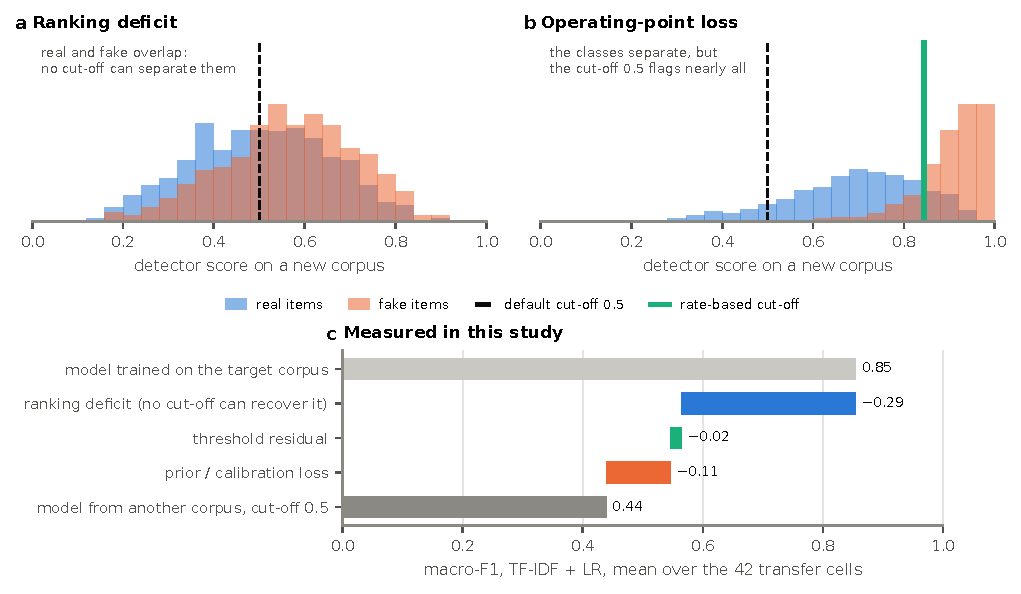
\includegraphics[width=\linewidth]{fig_concept}
\caption{Two ways a detector can fail on a new corpus. (a)~A ranking deficit: real and fake items receive overlapping scores, so no cut-off separates them. (b)~An operating-point loss: the scores separate the classes, but the cut-off learned on the training corpus (0.5) flags almost every item; a cut-off chosen by rate recovers most of the loss. Panels a and b use illustrative simulated scores. (c)~The measured decomposition of Eq.~\eqref{eq:decomp} for TF-IDF with logistic regression, averaged over the 42 transfer cells and five seeds.}\label{fig:concept}
\end{figure}

Two details of Eq.~\eqref{eq:decomp} could bias the split, and we check both. First, the ranking term compares the transfer oracle with the in-domain model at its \emph{default} threshold, so it also contains the in-domain threshold slack $F_{BB}(\tau^\star_{BB})-F_{BB}(\tau_0)$. Second, $\tau^\star$ is chosen on the same items it is scored on, which flatters $F_{AB}(\tau^\star)$ on small test sets and so inflates the operating-point share. We report the slack, and we recompute the decomposition with a \emph{cross-fitted} oracle, whose threshold is tuned on a random half of the target test set and scored on the other half (five repeats, both halves). We also repeat the decomposition with balanced accuracy, which, unlike macro-F1, does not depend on the class prior.

\subsection{Label-free operating points}\label{sec:oprepair}
We compare four ways of choosing a threshold without target labels.
(a)~\emph{EM prior adaptation} \citep{saerens2002adjusting} re-estimates the target prior from the source-calibrated posteriors by expectation--maximisation, adjusts the posteriors and thresholds them at 0.5. With Platt-calibrated scores this is the bias-corrected recipe recommended by \citet{alexandari2020labelshift}, and it is optimal under pure label shift.
(b)~\emph{Rate transfer} sets the threshold so that the share of target items flagged equals the source base rate $\pi_A$. It transfers the model's ranking-based decision rule rather than its score scale. We also report the variant that flags the share $q_A$ the source model flags on its own held-out test split.
(c)~\emph{Adjusted classify-and-count} \citep{forman2008quantifying} estimates the target prior as $\hat\pi_B=(\hat r_B-\mathrm{FPR}_A)/(\mathrm{TPR}_A-\mathrm{FPR}_A)$, where $\hat r_B$ is the share of target items above 0.5 and the error rates come from the source test split, and then flags the top $\hat\pi_B$ of target items.
(d)~A \emph{two-component Gaussian mixture} on the target logits places the threshold where the components' posteriors cross.
As references, we report the share $0.5$, which needs no information at all, and the true target prior $\pi_B$, which needs one number about the target but no item labels.

Rate transfer is a quantile threshold, and quantile thresholds are an old idea in quantification \citep{forman2008quantifying}. We do not claim the rule as new. What matters here is \emph{when} it should beat EM, and that can be stated exactly. Let $F^A_y$ and $F^B_y$ be the distributions of the source model's scores for class $y$ on source and target.

\begin{proposition}\label{prop:rate}
Suppose (i) there is a strictly increasing map $g$ with $F^B_y(g(u))=F^A_y(u)$ for both classes and all $u$, and (ii) $\pi_B=\pi_A$. Then flagging the top $q_A$ share of target items reproduces on $B$ the true- and false-positive rates that the threshold $\tau_0$ has on $A$, whereas the fixed threshold $\tau_0$ does so only if $g(\tau_0)=\tau_0$. If instead $g$ is the identity and $\pi_B\neq\pi_A$ (pure label shift), EM prior adaptation with calibrated scores is consistent and rate transfer is not.
\end{proposition}

The proof is in \ref{app:proof}. The two rules thus suit two different kinds of shift. EM assumes the score distributions within each class stay fixed while the class balance changes. Rate transfer assumes the reverse: the class balance stays roughly fixed while the scores are distorted by an order-preserving map. When the distortion is not order-preserving, part of the loss becomes a ranking deficit that no threshold can recover, which is the first term of Eq.~\eqref{eq:decomp}. Section~\ref{sec:op} checks which assumption our corpora come closer to, and a controlled experiment maps what happens when (ii) fails: each target test set is resampled (1{,}000 items, three draws) to a base rate of $\pi_A+\delta$ for $\delta\in\{-0.3,\dots,0.3\}$, clipped to $[0.05,0.95]$, and every operating point is recomputed.

\subsection{Mechanism probes}\label{sec:probes}
To identify what signal carries in-domain performance, we use eight probes, each run with \textsc{tfidf-lr} unless stated:
\emph{surface statistics only} (\textsc{style-gb} above);
\emph{group-only}, out-of-fold smoothed target encoding of group identity (publisher domain for PolitiFact, GossipCop and BanglaBait; speaker for LIAR; event for PHEME), i.e.\ how well the label is predicted by \emph{who} published an item;
\emph{learning curves} from 32 training items to the full split;
\emph{top-$K$ deletion}, removing the $K\in\{10,\dots,3000\}$ highest-$|w|$ features and retraining \citep[cf.][]{verma2026audit};
\emph{masking} of source tags and datelines, of time expressions and numbers, of named entities (spaCy \texttt{en\_core\_web\_sm}), or of all three;
\emph{topic-balanced training}, where classes are subsampled to equal size inside each of 50 $k$-means topic clusters, removing topic--label correlation from the training set;
\emph{corpus separability}, the proxy $\mathcal{A}$-distance $2(1-2\epsilon)$ between two corpora, with $\epsilon$ the cross-validated error of a classifier that tells them apart from text alone \citep{bendavid2010theory};
and \emph{feature attribution}, the largest-weight n-grams per class and their linear-SHAP magnitudes $|w_j|\,\mathbb{E}|x_j-\bar x_j|$.
For the more expensive probes (top-$K$, masking, vocabulary ablation) training is capped at 4{,}000 and test at 1{,}500 items; masking and vocabulary ablation use three seeds.

\subsection{Representation repairs}\label{sec:repair}
The ranking deficit can only be reduced by a better representation. We test repairs in a leave-one-corpus-out (LOCO) setting: for each held-out veracity corpus, the model is trained on the union of the other six (each capped at 1{,}500 training and 300 validation items) and evaluated on the held-out test split, with near-duplicates of any training corpus removed. Methods are: \emph{pooled} training; pooled training with sample weights that equalise every (corpus, class) cell (\emph{balanced}); balanced training on texts with source tags, datelines, URLs, handles and time expressions \emph{masked}; balanced training after deleting the 2{,}000 features most predictive of \emph{corpus identity} (from a one-vs-rest corpus classifier); and three dense variants on a 300-d SVD of the TF-IDF space: the SVD baseline, \emph{INLP} \citep{ravfogel2020inlp}, which projects out 15 iterations of linear corpus-identity directions, and \emph{CORAL} \citep{sun2016coral}, which aligns source feature covariance to the (unlabelled) target. None uses target labels; CORAL alone uses unlabelled target text.

We also re-implement three published generalisation methods for fake-news detection on one shared backbone, the frozen RoBERTa vectors of the 1{,}500-item subsets, in the same leave-one-corpus-out design (three seeds): EANN-style adversarial training, in which a corpus discriminator behind a gradient-reversal layer removes corpus information from a two-layer encoder \citep{wang2018eann,ganin2016dann}; an MDFEND-style mixture of five expert networks combined by a learned gate \citep{nan2021mdfend}, fed the text vector because the domain of a new corpus is unknown; and ENDEF-style entity debiasing, in which an entity-only model over the named entities found by spaCy is trained jointly with the main model and dropped at test time \citep{zhu2022endef}. Pooled logistic regression and a pooled two-layer network on the same vectors are the references. All networks are trained with AdamW and early stopping on pooled validation AUC.
